\documentclass[11pt,letterpaper]{article}
\usepackage[T1]{fontenc}
\usepackage{lmodern}
\usepackage[margin=0.8in,headheight=15pt]{geometry}
\usepackage{amsmath,amssymb,booktabs,array,xcolor,tikz,fancyhdr}
\usepackage[hidelinks]{hyperref}
\usetikzlibrary{arrows.meta}
\definecolor{ink}{HTML}{16384B}
\definecolor{accent}{HTML}{087E8B}
\definecolor{pale}{HTML}{EFF6F8}
\pagestyle{fancy}\fancyhf{}
\fancyhead[L]{\small\textcolor{ink}{Electromagnetism foundations}}
\fancyhead[R]{\small Learning note}
\fancyfoot[L]{\footnotesize Updated 6 October 2026}
\fancyfoot[R]{\thepage}
\setlength{\parindent}{0pt}\setlength{\parskip}{5pt}
\setlength{\emergencystretch}{2em}
\newcolumntype{P}[1]{>{\raggedright\arraybackslash}p{#1}}
\newcommand{\vect}[1]{\boldsymbol{#1}}
\newcommand{\dd}{\,\mathrm d}
\newcommand{\idea}[1]{\par\smallskip\noindent\colorbox{pale}{\parbox{\dimexpr\linewidth-2\fboxsep\relax}{\textbf{Physical meaning.} #1}}\par\smallskip}
\newcommand{\topic}[2]{\section{#1}\textit{#2}\par}
\newcommand{\reading}[1]{\par\smallskip{\small\textcolor{ink}{Further reading:} #1}\par}
\hypersetup{pdftitle={Electromagnetism Foundations: Fields, Flux, Divergence and Curl},pdfauthor={Learning-Note},pdfsubject={Physical meaning and operational measurement}}
\begin{document}
\begin{center}
{\LARGE\bfseries\color{ink} Electromagnetism Foundations}\\[6pt]
{\large Electric and magnetic fields; flux, divergence, and curl}\\[6pt]
{\small Updated 6 October 2026}
\end{center}

\section*{Purpose and reading order}
This note records established definitions, their physical interpretations, and representative experiments and applications. It distinguishes a \emph{definition}, a \emph{mathematical theorem}, and a \emph{physical law}. An illustration explains a definition; it does not prove a physical law.

The scope is the meaning and measurement of $\vect E$ and $\vect B$, the uses of flux, divergence, and curl, and a few laws that use them. The electromagnetic laws near the end are a reference map. A systematic lesson on Maxwell's equations, wave propagation, transmission-line reflection, and the AN720 antenna comes later.

\subsection*{What a field describes}
A field assigns a value to each position and time. Temperature $T(\vect r,t)$ is a scalar field. Electric field $\vect E(\vect r,t)$, magnetic field $\vect B(\vect r,t)$, and fluid velocity $\vect v(\vect r,t)$ are vector fields. A vector field assigns both magnitude and direction.

Field arrows and field lines are drawings that summarize a field. They are not material threads, and a field need not be a flow of matter. A field can exist without a measuring probe at the point of interest.

\subsection*{Three levels of statement}
\begin{description}
\item[Definition:] Flux is the integral of a field's perpendicular component over an oriented surface.
\item[Theorem:] The divergence theorem relates closed-surface flux to the volume integral of divergence, under suitable regularity conditions.
\item[Physical law:] Gauss's electric law relates electric flux to enclosed charge. Geometry alone does not establish that relationship.
\end{description}

\subsection*{Notation and assumptions}
$\hat{\vect n}$ is a unit surface normal, $d\vect A=\hat{\vect n}\,dA$, and $d\vect\ell$ is a directed line element. $\partial V$ is the boundary of volume $V$; $\partial S$ is the boundary of surface $S$. A closed-surface normal points outward. Loop orientation follows the right-hand rule relative to its surface normal.

Classical fields and SI units are used. Point-charge forces refer to an external field, excluding the probe's own field. Differential formulas assume smooth fields where evaluated; ideal point charges and surface discontinuities require integral laws or distributional treatment. All field measurements refer to a specified reference frame.

\reading{Field definitions: \cite{electric,magnetic}. Vector-field framework: \cite{vectorfields}.}

\newpage
\topic{Electric field: force per unit charge}{Separate the property of the environment from the particular charge used to test it.}

\subsection*{Operational definition}
For a sufficiently small test charge at rest in the chosen frame, after excluding other forces,
\begin{equation}
\vect E(\vect r,t)=\lim_{q\to0}\frac{\vect F_E(\vect r,t;q)}{q}.
\end{equation}
The limit expresses negligible disturbance of the source arrangement. In ordinary measurements the probe need only be small enough for that disturbance to be negligible. The denominator is signed charge: a negative probe feels a force opposite to $\vect E$. Units are $\mathrm{N/C}=\mathrm{V/m}$.

\idea{The electric field tells us the force a unit positive charge would experience at that location and time. The probe reveals the field; it does not define the source arrangement into existence.}

\subsection*{What an experiment measures}
An ideal force-balance experiment places a probe of known charge in a field and balances its electric force against a calibrated mechanical force. If a charged object of mass $m$ is suspended with gravity and an upward electric force balanced, $qE=mg$. Measuring $m$ and $q$ determines $E$; measuring a known $E$ can instead determine $q$. Real experiments account for buoyancy, drag, and probe size.

In a beam-deflection measurement, a particle of known charge and mass passes through a nearly uniform transverse electric field. Neglecting magnetic fields and collisions,
\[
a_y=\frac{qE_y}{m},\qquad y=\frac{qE_y}{2m}\,t^2
\]
for zero initial transverse velocity. Measuring the displacement and transit time determines the field. This is a force measurement through the resulting motion.

\subsection*{Concrete example}
If $\vect E=200\,\hat{\vect y}\ \mathrm{N/C}$, a $+1\,\mathrm{nC}$ probe feels $2\times10^{-7}\,\hat{\vect y}\ \mathrm N$. A $-1\,\mathrm{nC}$ probe feels the opposite force. Changing the probe changes the force; it does not change the undisturbed field being measured.

\subsection*{What this definition does not say}
It does not specify how $\vect E$ is produced. Static charges produce electric fields; changing magnetic fields can also be associated with electric fields. Those are statements about physical laws, not consequences of dividing force by charge.

In electrostatics, $\vect E=-\nabla\phi$ and the potential difference is $\Delta\phi=-\int\vect E\cdot d\vect\ell$. A voltmeter can support field inference in a known electrostatic geometry. In a general time-varying situation, an electric-field line integral can depend on the path, so an arbitrary field cannot be reconstructed from a single voltage reading.

\reading{Operational field definition and test-charge independence: \cite{electric}. The force-balance and beam examples here are idealized applications of $\vect F_E=q\vect E$.}

\newpage
\topic{Magnetic field: velocity-dependent force}{Measure how force changes when a known charge moves with different velocities.}

\subsection*{Force law and measurement}
For an ideal point charge in an external classical electromagnetic field,
\begin{equation}
\vect F=q\bigl(\vect E+\vect v\times\vect B\bigr),\qquad
\vect F_B=q\vect v\times\vect B.
\end{equation}
The electric contribution can be determined separately, for example with a probe instantaneously at rest. The remaining velocity-dependent force determines $\vect B$. This is the operational route to magnetic-field measurement, using the experimentally established Lorentz-force relationship.

The force magnitude is $F_B=|q|vB\sin\theta$, where $\theta$ is the angle between $\vect v$ and $\vect B$. Thus $B=F_B/(|q|v)$ only for perpendicular motion. The SI unit is the tesla: $1\,\mathrm T=1\,\mathrm{N\,s/(C\,m)}$.

\idea{Magnetic field describes a velocity-dependent sideways force on a charge. The force is perpendicular to both velocity and field. The field itself need not be perpendicular to velocity.}

\subsection*{Why one velocity is insufficient}
Motion parallel to $\vect B$ gives zero magnetic force even when $B\ne0$. More generally, one velocity direction cannot reveal the component of $\vect B$ parallel to that velocity. Measurements with nonparallel velocities can determine the full field vector. For positive charge, the force direction follows $\vect v\times\vect B$; negative charge reverses it.

\subsection*{Beam-curvature experiment}
In a uniform field, with negligible electric field and initial motion perpendicular to $\vect B$, a nonrelativistic charged particle follows a circle. Magnetic force supplies the centripetal force:
\[
|q|vB=\frac{mv^2}{r},\qquad B=\frac{mv}{|q|r}.
\]
For an electron with $v=10^6\,\mathrm{m/s}$ and $r=0.01\,\mathrm m$, this gives approximately $5.69\times10^{-4}\,\mathrm T$. The measured bending direction determines the field orientation once the charge sign is known. At relativistic speeds, use momentum: $r=p/(|q|B)$.

\subsection*{Other probes and energy}
A current loop experiences magnetic torque; a Hall probe measures a transverse voltage caused by magnetic deflection of charge carriers. These are different experimental access routes to the same field.

For the translational Lorentz magnetic force on a point charge,
\[
\vect F_B\cdot\vect v=q(\vect v\times\vect B)\cdot\vect v=0.
\]
It changes direction without directly changing the particle's kinetic energy. This result does not prohibit a magnetic dipole from exchanging interaction energy with an external field.

\reading{Magnetic force and particle trajectories: \cite{magnetic}. Current-loop measurement: \cite{torque}.}

\newpage
\topic{Spin, magnetic moments, and stationary magnets}{Distinguish a magnetic property of an object from the field in the space around it.}

\subsection*{Magnetic moment and spin}
A magnetic dipole moment $\vect\mu$ describes dipole strength and orientation, with units $\mathrm{A\,m^2}=\mathrm{J/T}$. A small planar current loop has $\vect\mu=IA\hat{\vect n}$. A particle can also have an intrinsic magnetic moment.

Electron spin is intrinsic angular momentum, not literal rotation of a charged sphere. It is present even without centre-of-mass motion. For electron spin angular momentum $\vect S$,
\[
\vect\mu_s=-g_e\frac{e}{2m_e}\vect S,
\]
where $e>0$ and $g_e$ is close to $2$. The negative sign makes the spin magnetic moment opposite to the spin angular momentum. Orbital angular momentum can also contribute to an atom's magnetic moment.

\textbf{Experimental access.} Atomic beam splitting in a nonuniform magnetic field (Stern--Gerlach-type experiments) reveals discrete magnetic-moment projections; an atomic beam is not a direct beam of free electrons. Spectroscopy and electron spin resonance probe spin-related magnetic energy splittings. Quantum theory supplies quantitative predictions. There is no established internal rotating-ball mechanism underlying electron spin.\cite{spin,spinmatter}

\subsection*{Why a stationary magnet can respond}
A stationary structureless point charge has zero translational magnetic Lorentz force. A stationary magnet has magnetic moments, so it can experience torque or force. For an ideal small permanent dipole with fixed moment in an imposed field $\vect B_{\rm ext}$,
\begin{equation}
\vect\tau=\vect\mu\times\vect B_{\rm ext},\quad
U=-\vect\mu\cdot\vect B_{\rm ext},\quad
\vect F=\nabla(\vect\mu\cdot\vect B_{\rm ext}).
\end{equation}
The field must vary slowly over the dipole's size. A uniform field can turn a misaligned moment but gives no net force on this ideal dipole. A spatially varying field can give a force. Induced or changing moments require a material-response treatment; these fixed-moment formulas cannot be applied unchanged.\cite{torque,dipolegradient}

\subsection*{Permanent magnets and energy}
Electronic moments can cancel, so not every atom or material has a net magnetic moment. Ferromagnetic domains contain ordered moments; a permanent magnet retains a net magnetization when the domain arrangement has an uncancelled resultant. Alignment is governed by material interactions, including quantum exchange, and need not mean every moment in the object points identically.\cite{domains}

Having spin or maintaining a static permanent-magnet field does not continuously consume energy. State transitions can exchange energy without an electron slowing a literal rotation. When magnets move toward a lower-energy configuration, interaction energy can become mechanical energy. Reversing that motion requires work in the corresponding ideal reversible case. A resistive electromagnet needs power to replace resistive losses; a static field itself is not a continuous expenditure.\cite{spin,magenergy}

\newpage
\topic{Flux: combine a field over a surface}{Answer a total-crossing question, rather than a question about one point.}

\subsection*{Definition and orientation}
For an oriented surface $S$ and vector field $\vect F$,
\begin{equation}
\Phi_F=\int_S\vect F\cdot\hat{\vect n}\dd A.
\end{equation}
For a flat surface of area $A$ in a uniform field,
\[
\Phi_F=FA\cos\theta,
\]
where $\theta$ is measured from the \emph{normal}, not from the surface. Reversing the normal reverses the sign. Tangential components contribute nothing. For a closed surface, use the outward normal and add all inward and outward contributions with their signs.

\begin{center}
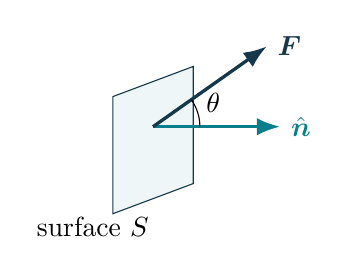
\begin{tikzpicture}[>=Latex,scale=0.85]
\filldraw[fill=pale,draw=ink] (0,-1.1)--(1.2,-0.65)--(1.2,1.1)--(0,0.65)--cycle;
\draw[->,very thick,accent] (0.6,0.2)--(2.5,0.2) node[right] {$\hat{\vect n}$};
\draw[->,very thick,ink] (0.6,0.2)--(2.3,1.4) node[right] {$\vect F$};
\draw (1.3,0.2) arc[start angle=0,end angle=35,radius=0.7];
\node at (1.5,0.55) {$\theta$};
\node at (-0.3,-1.3) {surface $S$};
\end{tikzpicture}
\end{center}

\idea{Flux adds the perpendicular field contributions over a surface. It represents actual transport only when the chosen field describes a transported quantity.}

\subsection*{Common uses and units}
\begin{center}\small
\begin{tabular}{P{0.24\linewidth}P{0.39\linewidth}P{0.22\linewidth}}
\toprule
Integrated field & Meaning of the surface integral & Units\\\midrule
Fluid velocity $\vect v$ & Signed volume flow rate & $\mathrm{m^3/s}$\\
Mass flux density $\rho\vect v$ & Signed mass flow rate & $\mathrm{kg/s}$\\
Heat flux density $\vect q_h$ & Heat-transfer rate & $\mathrm W$\\
Current density $\vect J$ & Electric current & $\mathrm A$\\
Electric field $\vect E$ & Electric flux & $\mathrm{N\,m^2/C}$\\
Magnetic field $\vect B$ & Magnetic flux & $\mathrm{Wb=T\,m^2}$\\\bottomrule
\end{tabular}\end{center}
Electric and magnetic flux are not rates of field substance passing through a surface. They are geometrical integrals. Their physical significance comes from laws that relate them to charge or induced emf.

\subsection*{Illustrative calculation}
Uniform water velocity $0.5\,\mathrm{m/s}$ perpendicular to a $0.02\,\mathrm{m^2}$ opening gives $0.01\,\mathrm{m^3/s}=10\,\mathrm{L/s}$. A magnetic field $0.1\,\mathrm T$ perpendicular to a $0.02\,\mathrm{m^2}$ loop gives $0.002\,\mathrm{Wb}$. These are the same geometrical operation with different physical inputs and units.

\reading{Field and surface-integral interpretation: \cite{vectorfields}. Magnetic-flux application: \cite{faraday}.}

\newpage
\topic{Divergence: local outward balance}{Distinguish movement through a region from net removal or supply within it.}

\subsection*{Definition}
At a point, divergence is net outward flux from a shrinking enclosing volume, divided by that volume:
\begin{equation}
\nabla\cdot\vect F
=\lim_{\Delta V\to0}\frac{1}{\Delta V}
\oint_{\partial(\Delta V)}\vect F\cdot\hat{\vect n}\dd A
=\frac{\partial F_x}{\partial x}+\frac{\partial F_y}{\partial y}+\frac{\partial F_z}{\partial z}.
\end{equation}
It is a scalar with units of $F$ divided by length. Positive divergence means a local net outward balance; negative divergence means a net inward balance. Zero divergence permits a nonzero, spatially varying field.

\idea{For a transport field, divergence tells us whether the local flow carries more out than in. A conservation law then tells us whether that imbalance changes stored quantity or is supplied by an internal source.}

\subsection*{Three illustrative fields}
For uniform motion $\vect v=U\hat{\vect x}$, $\nabla\cdot\vect v=0$: a small box has equal total inflow and outflow. For planar expansion $\vect v=a(x\hat{\vect x}+y\hat{\vect y})$, $\nabla\cdot\vect v=2a$: a moving small area expands. For three-dimensional expansion $\vect v=a\vect r$, divergence is $3a$.

For a small material volume transported by a smooth velocity field,
\[
\frac{1}{\Delta V}\frac{D(\Delta V)}{Dt}=\nabla\cdot\vect v.
\]
Velocity divergence measures local fractional volume expansion. Density accumulation in a \emph{fixed} region instead depends on divergence of the \emph{mass flux} $\rho\vect v$. These are related but different statements.

\subsection*{Common uses}
Mass and charge conservation connect divergence of a transport field to a time change of density. Heat balance connects divergence of heat flux to local energy storage. In electrostatics, Gauss's law connects electric divergence to charge density. These uses work because each needs a local balance, not merely a field magnitude.

\subsection*{The divergence theorem is mathematics}
For a suitable smooth field and volume,
\begin{equation}
\oint_{\partial V}\vect F\cdot\hat{\vect n}\dd A
=\int_V\nabla\cdot\vect F\dd V.
\end{equation}
The theorem relates a whole-boundary measurement to local measurements throughout the interior. It does not say what produces the field. No charge law, heat law, or fluid law follows from it alone.

\reading{Definitions and applications: \cite{calculus,gauss}.}

\newpage
\topic{Curl: distinguish local rotation from simple movement}{Compare neighboring vectors; one vector at one point cannot reveal local circulation.}

\subsection*{Circulation and curl}
Circulation is a field's tangential contribution summed along a closed path:
\[
\Gamma_F=\oint_C\vect F\cdot d\vect\ell.
\]
For a small planar loop centred near a point, the normal component of curl is
\begin{equation}
(\nabla\times\vect F)\cdot\hat{\vect n}
=\lim_{\Delta A\to0}\frac{1}{\Delta A}
\oint_{\partial(\Delta S)}\vect F\cdot d\vect\ell.
\end{equation}
Curl is a vector with units of $F$ divided by length. Its direction specifies an oriented circulation axis. Curling the right-hand fingers around the positive loop direction makes the thumb point along $\hat{\vect n}$.

In Cartesian coordinates,
\[
\nabla\times\vect F=
\left(\frac{\partial F_z}{\partial y}-\frac{\partial F_y}{\partial z}\right)\hat{\vect x}
+\left(\frac{\partial F_x}{\partial z}-\frac{\partial F_z}{\partial x}\right)\hat{\vect y}
+\left(\frac{\partial F_y}{\partial x}-\frac{\partial F_x}{\partial y}\right)\hat{\vect z}.
\]

\idea{For fluid velocity, curl measures local rotational tendency. For a general field, it measures local circulation; it does not imply that material is physically spinning.}

\subsection*{Rotation can occur with straight flow arrows}
Take $x$ rightward and $y$ upward, with $\vect v=ay\hat{\vect x}$ and $a>0$. Upper layers move rightward faster than lower layers. A small freely carried spherical marker has a clockwise rotational tendency:
\[
\nabla\times\vect v=-a\hat{\vect z},\qquad
\vect\Omega_{\rm local}=\tfrac12\nabla\times\vect v.
\]
The flow also deforms material. The half-curl describes the rotational part of the local velocity gradient, not necessarily the rotation rate of every arbitrarily shaped immersed object.

\subsection*{Pure rotation provides a calibration}
For rigid rotation $\vect v=\vect\Omega\times\vect r$ with constant $\vect\Omega$, $\nabla\times\vect v=2\vect\Omega$. Uniform translation has zero curl. Fluid mechanics calls velocity curl \emph{vorticity}; it is used to characterize shear and vortices.

\subsection*{Stokes' theorem is mathematics}
\[
\oint_{\partial S}\vect F\cdot d\vect\ell
=\int_S(\nabla\times\vect F)\cdot\hat{\vect n}\dd A.
\]
This relates boundary circulation to curl over a spanning surface. Electromagnetic laws specify what that circulation is related to physically. For example, induction links electric circulation to changing magnetic flux; that link is not part of the curl definition.

\reading{Vector calculus and fluid interpretations: \cite{calculus}. Induction application: \cite{faraday}.}

\newpage
\topic{Compare the operations without conflating them}{A field can vary without having divergence or curl.}

\subsection*{Simple planar velocity fields}
Treat these as three-dimensional fields with zero $z$ component and no $z$ dependence. $U$ is constant speed; $a$ and $\Omega$ have units $\mathrm{s^{-1}}$.
\begin{center}\small
\begin{tabular}{P{0.34\linewidth}P{0.16\linewidth}P{0.20\linewidth}P{0.18\linewidth}}
\toprule
Velocity field & Divergence & Curl & Local behavior\\\midrule
$U\hat{\vect x}$ & $0$ & $\vect0$ & Translation\\[3pt]
$a(x\hat{\vect x}+y\hat{\vect y})$ & $2a$ & $\vect0$ & Expansion\\[3pt]
$\Omega(-y\hat{\vect x}+x\hat{\vect y})$ & $0$ & $2\Omega\hat{\vect z}$ & Rigid rotation\\[3pt]
$ay\hat{\vect x}$ & $0$ & $-a\hat{\vect z}$ & Shear with rotation\\[3pt]
$a(x\hat{\vect x}-y\hat{\vect y})$ & $0$ & $\vect0$ & Area-preserving strain\\\bottomrule
\end{tabular}\end{center}
The last row stretches material in one direction and compresses it in another. Thus zero divergence and zero curl together do not imply a uniform field or an absence of deformation.

\subsection*{Why circular field lines are not enough}
For a long straight wire carrying steady current $I$, the vacuum magnetic field outside the wire is
\[
\vect B=\frac{\mu_0 I}{2\pi r}\hat{\vect\phi}.
\]
A circular path enclosing the wire has circulation $\mu_0 I$. Yet a sufficiently small loop entirely in the current-free exterior has zero circulation, and $\nabla\times\vect B=\vect0$ there.

There is no conflict with Stokes' theorem. A surface spanning the enclosing circle must account for the wire's current-carrying region (or, in the ideal zero-radius model, its singularity). One cannot apply the current-free exterior formula as a smooth field everywhere on that surface.\cite{ampere}

\subsection*{Why strong field is not enough}
Between large oppositely charged plates, away from edges and charges, an approximately uniform electrostatic field has zero divergence and zero curl. The field can still exert a large force on a test charge. Field magnitude, local outward balance, and local circulation answer different questions.

\subsection*{Historical relationship to physics}
There was no universal sequence in which all three finished definitions preceded their applications. Mathematical tools and physical questions developed together. Maxwell's 1871 classification discussed flux in fluids, heat, and electricity, introduced the name \emph{curl}, and used \emph{convergence} with the opposite sign to modern divergence. These were shared mathematical structures across subjects, including electromagnetism.\cite{history}

Logical dependence is clearer than historical chronology: define an operation; independently specify a physical law involving it; use mathematical theorems to obtain equivalent forms. An operation's definition neither proves nor requires an electromagnetic law.

\newpage
\topic{Physical laws using flux and divergence}{A balance law supplies the physics that a geometrical operation does not.}

\subsection*{Mass conservation}
For a fixed volume, with no mass sources or sinks,
\begin{equation}
\frac{d}{dt}\int_V\rho\dd V
=-\oint_{\partial V}\rho\vect v\cdot\hat{\vect n}\dd A,
\qquad
\frac{\partial\rho}{\partial t}+\nabla\cdot(\rho\vect v)=0.
\end{equation}
\textbf{Physical content:} mass lost from the interior must leave through its boundary. \textbf{Mathematical role:} flux measures boundary transport; the divergence theorem converts that transport into a local balance.

For constant-density incompressible flow, $\nabla\cdot\vect v=0$. Water can accelerate through a narrowing pipe while preserving mass: $\rho A_1v_1=\rho A_2v_2$ for steady uniform cross-sectional flow. Faster downstream flow alone does not imply positive divergence.

\subsection*{Charge conservation}
For total charge density $\rho_q$ and its consistent current density $\vect J$,
\begin{equation}
\frac{d}{dt}\int_V\rho_q\dd V
=-\oint_{\partial V}\vect J\cdot\hat{\vect n}\dd A,
\qquad
\frac{\partial\rho_q}{\partial t}+\nabla\cdot\vect J=0.
\end{equation}
\textbf{Physical content:} local charge cannot disappear; a boundary current changes the charge inside. \textbf{Use:} if more positive-charge current enters a small conductor region than leaves, positive charge accumulates there. This is distinct from Gauss's electric law, which relates charge to the electric field.

\subsection*{Heat conduction and energy balance}
For a stationary solid with constant density $\rho$, specific heat $c$, heat flux density $\vect q_h$, and volumetric heat input $s_h$,
\begin{equation}
\rho c\frac{\partial T}{\partial t}=-\nabla\cdot\vect q_h+s_h.
\end{equation}
This reduced model excludes bulk material motion, mechanical work, and phase-change terms. Positive outward heat-flux divergence removes thermal energy locally. A heater can compensate through $s_h$.

For an isotropic material obeying Fourier's conduction law, $\vect q_h=-k\nabla T$. For constant conductivity $k$ and zero input,
\[
\rho c\frac{\partial T}{\partial t}=k\nabla^2T.
\]
Here $\nabla T$ gives the spatial temperature slope and $\nabla^2T=\nabla\cdot\nabla T$. Fourier's law is a material law; it is not a theorem about flux. The balance equations above follow by applying conservation to a fixed volume and then using the divergence theorem.

\reading{Heat-flow framework: \cite{vectorfields}. Charge continuity and its electromagnetic consistency: \cite{maxwell}.}

\newpage
\topic{Electromagnetic laws: a limited reference map}{Read what each law links, without beginning the full Maxwell-equation lesson.}

\subsection*{Electric flux and charge}
In vacuum, or using total charge including bound charge in the microscopic formulation,
\begin{equation}
\oint_{\partial V}\vect E\cdot\hat{\vect n}\dd A
=\frac{Q_{\rm enclosed}}{\epsilon_0},\qquad
\nabla\cdot\vect E=\frac{\rho_q}{\epsilon_0}.
\end{equation}
This is Gauss's electric law. Symmetry makes it useful for calculating fields around spheres, cylinders, and planes. It is a physical relationship between charge and field, not the definition of flux or divergence.\cite{gauss}

\subsection*{Magnetic flux has zero closed-surface total}
Standard classical electromagnetism has
\begin{equation}
\oint_{\partial V}\vect B\cdot\hat{\vect n}\dd A=0,
\qquad \nabla\cdot\vect B=0.
\end{equation}
This expresses the absence of magnetic monopole sources in the standard theory; isolated magnetic monopoles have not been experimentally established. Magnetic field is not required to vanish. A surface around one end of a bar magnet also cuts through the magnet: outgoing flux is balanced by incoming flux.\cite{maxwell}

\subsection*{Changing magnetic flux and electric circulation}
For a stationary loop and its fixed spanning surface,
\begin{equation}
\mathcal E=\oint_{\partial S}\vect E\cdot d\vect\ell
=-\frac{d}{dt}\int_S\vect B\cdot\hat{\vect n}\dd A,
\qquad \nabla\times\vect E=-\frac{\partial\vect B}{\partial t}.
\end{equation}
Faraday's law is tested through induced emf when linked magnetic flux changes. A conducting loop makes the effect measurable, but the induced electric field can exist without that conductor. Moving-loop problems also require the motional contribution $\vect v\times\vect B$.\cite{faraday}

\subsection*{Steady current and magnetic circulation}
For steady currents in vacuum, or consistently using total microscopic current,
\begin{equation}
\oint_{\partial S}\vect B\cdot d\vect\ell=\mu_0 I_{\rm through\ S},
\qquad \nabla\times\vect B=\mu_0\vect J.
\end{equation}
This magnetostatic form of Ampere's law is useful for long wires and solenoids. It is insufficient for general time-dependent fields: Maxwell's additional electric-field time-derivative term will be studied next.\cite{ampere,maxwell}

\textbf{Scope boundary.} These laws identify why flux, divergence, and curl are useful in electromagnetism. Their experimental development, displacement current, and mutually coupled dynamics belong to the next lesson. None of the mathematical definitions alone establishes these physical equalities.

\newpage
\section*{References and source map}
The prose, examples, and calculations in this note are original explanations. Sources below support the standard definitions and physical statements. Equations are stated with their model assumptions; mechanical pictures of quantum spin are excluded. Links were checked on 2 October 2026.

\begingroup\small
\raggedright
\begin{thebibliography}{99}
\bibitem{electric} OpenStax, \emph{University Physics, Volume 2}, Sec. 5.4, ``Electric Field.''
\url{https://openstax.org/books/university-physics-volume-2/pages/5-4-electric-field}
\bibitem{magnetic} OpenStax, \emph{University Physics, Volume 2}, Sec. 11.2, ``Magnetic Fields and Lines.''
\url{https://openstax.org/books/university-physics-volume-2/pages/11-2-magnetic-fields-and-lines}
\bibitem{torque} OpenStax, \emph{University Physics, Volume 2}, Sec. 11.5, ``Force and Torque on a Current Loop.''
\url{https://openstax.org/books/university-physics-volume-2/pages/11-5-force-and-torque-on-a-current-loop}
\bibitem{spin} OpenStax, \emph{University Physics, Volume 3}, Sec. 8.3, ``Electron Spin.''
\url{https://openstax.org/books/university-physics-volume-3/pages/8-3-electron-spin}
\bibitem{spinmatter} R. P. Feynman, R. B. Leighton, and M. Sands, \emph{The Feynman Lectures on Physics}, Vol. II, Ch. 34, ``The Magnetism of Matter.''
\url{https://www.feynmanlectures.caltech.edu/II_34.html}
\bibitem{dipolegradient} Feynman, Leighton, and Sands, Vol. II, Ch. 35, ``Paramagnetism and Magnetic Resonance.''
\url{https://www.feynmanlectures.caltech.edu/II_35.html}
\bibitem{domains} OpenStax, \emph{University Physics, Volume 2}, Sec. 12.7, ``Magnetism in Matter.''
\url{https://openstax.org/books/university-physics-volume-2/pages/12-7-magnetism-in-matter}
\bibitem{magenergy} OpenStax, \emph{University Physics, Volume 2}, Sec. 14.3, ``Energy in a Magnetic Field.''
\url{https://openstax.org/books/university-physics-volume-2/pages/14-3-energy-in-a-magnetic-field}
\bibitem{vectorfields} Feynman, Leighton, and Sands, Vol. II, Ch. 2, ``Differential Calculus of Vector Fields.''
\url{https://www.feynmanlectures.caltech.edu/II_02.html}
\bibitem{calculus} OpenStax, \emph{Calculus, Volume 3}, Sec. 6.5, ``Divergence and Curl.''
\url{https://openstax.org/books/calculus-volume-3/pages/6-5-divergence-and-curl}
\end{thebibliography}
\endgroup

\newpage
\section*{References and source map (continued)}
\begingroup\small
\raggedright
\begin{thebibliography}{99}\setcounter{enumiv}{10}
\bibitem{gauss} OpenStax, \emph{University Physics, Volume 2}, Sec. 6.3, ``Applying Gauss's Law.''
\url{https://openstax.org/books/university-physics-volume-2/pages/6-3-applying-gausss-law}
\bibitem{faraday} OpenStax, \emph{University Physics, Volume 2}, Sec. 13.1, ``Faraday's Law.''
\url{https://openstax.org/books/university-physics-volume-2/pages/13-1-faradays-law}
\bibitem{ampere} OpenStax, \emph{University Physics, Volume 2}, Sec. 12.5, ``Ampere's Law.''
\url{https://openstax.org/books/university-physics-volume-2/pages/12-5-amperes-law}
\bibitem{maxwell} OpenStax, \emph{University Physics, Volume 2}, Sec. 16.1, ``Maxwell's Equations and Electromagnetic Waves.''
\url{https://openstax.org/books/university-physics-volume-2/pages/16-1-maxwells-equations-and-electromagnetic-waves}
\bibitem{history} J. Clerk Maxwell, ``Remarks on the Mathematical Classification of Physical Quantities,'' \emph{Proceedings of the London Mathematical Society}, s1-3, 224--233 (1871). Primary historical source; terminology differs from modern usage.
\url{https://clerkmaxwellfoundation.org/MathematicalClassificationofPhysicalQuantities_Maxwell.pdf}
\end{thebibliography}
\endgroup

\subsection*{How to use the references}
References 1--3 support operational field definitions and classical probes. References 4--8 support the spin, magnetic-moment, material, and energy distinctions. References 9--10 support vector-field mathematics. References 11--14 support the electromagnetic-law map. Reference 15 records Maxwell's own terminology rather than assuming a simple historical ``mathematics first, physics later'' sequence.

\subsection*{Document maintenance}
This is a living note with a stable source filename. The companion \path{laws-experiments-and-timeline.tex} develops the experiments, EMF, and relationships among the physical laws introduced here. Later edits should update the topic document and PDF, add a dated entry to \texttt{../Documents/changes.tex}, and update \texttt{../Documents/plan.tex} when a learning step is completed or revised. No numbered releases or copied revision folders are needed.

\subsection*{Local and Overleaf compilation}
This topic is self-contained in \path{fields-and-vector-calculus.tex}: references and its vector diagram are embedded in the source. On a standard TeX Live installation, run the following from the topic folder:
\begin{verbatim}
pdflatex -interaction=nonstopmode -halt-on-error fields-and-vector-calculus.tex
pdflatex -interaction=nonstopmode -halt-on-error fields-and-vector-calculus.tex
\end{verbatim}
Two passes resolve references. No BibTeX, external images, shell escape, or machine-specific paths are required. For Overleaf, upload \path{fields-and-vector-calculus.tex} from this topic folder and choose pdfLaTeX. Uploading the PDF is optional; it is an output, not a build dependency. The two documents in \texttt{Documents/} compile independently with the same two-pass procedure.

\end{document}
